\PassOptionsToPackage{unicode=true}{hyperref} % options for packages loaded elsewhere
\PassOptionsToPackage{hyphens}{url}
%
\documentclass[ignorenonframetext,]{beamer}
\usepackage{pgfpages}
\setbeamertemplate{caption}[numbered]
\setbeamertemplate{caption label separator}{: }
\setbeamercolor{caption name}{fg=normal text.fg}
\beamertemplatenavigationsymbolsempty
% Prevent slide breaks in the middle of a paragraph:
\widowpenalties 1 10000
\raggedbottom
\setbeamertemplate{part page}{
\centering
\begin{beamercolorbox}[sep=16pt,center]{part title}
  \usebeamerfont{part title}\insertpart\par
\end{beamercolorbox}
}
\setbeamertemplate{section page}{
\centering
\begin{beamercolorbox}[sep=12pt,center]{part title}
  \usebeamerfont{section title}\insertsection\par
\end{beamercolorbox}
}
\setbeamertemplate{subsection page}{
\centering
\begin{beamercolorbox}[sep=8pt,center]{part title}
  \usebeamerfont{subsection title}\insertsubsection\par
\end{beamercolorbox}
}
\AtBeginPart{
  \frame{\partpage}
}
\AtBeginSection{
  \ifbibliography
  \else
    \frame{\sectionpage}
  \fi
}
\AtBeginSubsection{
  \frame{\subsectionpage}
}
\usepackage{lmodern}
\usepackage{amssymb,amsmath}
\usepackage{ifxetex,ifluatex}
\usepackage{fixltx2e} % provides \textsubscript
\ifnum 0\ifxetex 1\fi\ifluatex 1\fi=0 % if pdftex
  \usepackage[T1]{fontenc}
  \usepackage[utf8]{inputenc}
  \usepackage{textcomp} % provides euro and other symbols
\else % if luatex or xelatex
  \usepackage{unicode-math}
  \defaultfontfeatures{Ligatures=TeX,Scale=MatchLowercase}
\fi
% use upquote if available, for straight quotes in verbatim environments
\IfFileExists{upquote.sty}{\usepackage{upquote}}{}
% use microtype if available
\IfFileExists{microtype.sty}{%
\usepackage[]{microtype}
\UseMicrotypeSet[protrusion]{basicmath} % disable protrusion for tt fonts
}{}
\IfFileExists{parskip.sty}{%
\usepackage{parskip}
}{% else
\setlength{\parindent}{0pt}
\setlength{\parskip}{6pt plus 2pt minus 1pt}
}
\usepackage{hyperref}
\hypersetup{
            pdftitle={Risk},
            pdfborder={0 0 0},
            breaklinks=true}
\urlstyle{same}  % don't use monospace font for urls
\newif\ifbibliography
\usepackage{graphicx,grffile}
\makeatletter
\def\maxwidth{\ifdim\Gin@nat@width>\linewidth\linewidth\else\Gin@nat@width\fi}
\def\maxheight{\ifdim\Gin@nat@height>\textheight\textheight\else\Gin@nat@height\fi}
\makeatother
% Scale images if necessary, so that they will not overflow the page
% margins by default, and it is still possible to overwrite the defaults
% using explicit options in \includegraphics[width, height, ...]{}
\setkeys{Gin}{width=\maxwidth,height=\maxheight,keepaspectratio}
\setlength{\emergencystretch}{3em}  % prevent overfull lines
\providecommand{\tightlist}{%
  \setlength{\itemsep}{0pt}\setlength{\parskip}{0pt}}
\setcounter{secnumdepth}{0}

% set default figure placement to htbp
\makeatletter
\def\fps@figure{htbp}
\makeatother


\title{Risk}
\author{}
\date{\vspace{-2.5em}10/19/2020}

\begin{document}
\frame{\titlepage}

\begin{frame}{Today}
\protect\hypertarget{today}{}

\begin{itemize}
\tightlist
\item
  Discussion
\item
  Economics of Risk
\item
  Risk and Development
\end{itemize}

\end{frame}

\begin{frame}{Discussion: Part 1}
\protect\hypertarget{discussion-part-1}{}

In groups, discuss:

\begin{itemize}
\tightlist
\item
  What are the most important development problems caused by risk?
\end{itemize}

\end{frame}

\begin{frame}{Discussion: Part 1}
\protect\hypertarget{discussion-part-1-1}{}

Of the problems you identified:

\begin{itemize}
\tightlist
\item
  Which can be addressed by government? How?
\item
  Which can be addressed by the private sector? How?
\end{itemize}

\end{frame}

\hypertarget{economics-of-risk}{%
\section{Economics of Risk}\label{economics-of-risk}}

\begin{frame}{The St.~Petersburg Paradox}
\protect\hypertarget{the-st.petersburg-paradox}{}

A casino game:

\begin{itemize}
\tightlist
\item
  A coin is flipped at each stage
\item
  If heads, \$2 goes into pot on first flip
\item
  Each additional heads doubles the pot
\item
  First tails: game ends, collect pot contents
\end{itemize}

How much would you pay to play?

\end{frame}

\begin{frame}{The St.~Petersburg Paradox}
\protect\hypertarget{the-st.petersburg-paradox-1}{}

\[
E = \frac{1}{2}2+\frac{1}{4}4+\frac{1}{8}8 + \frac{1}{16}16+...=\infty
\] \ldots{} the expected value is infinite!

So why did nobody bid infinity or even a very large number?

\end{frame}

\begin{frame}{Daniel Bernoulli (1738)}
\protect\hypertarget{daniel-bernoulli-1738}{}

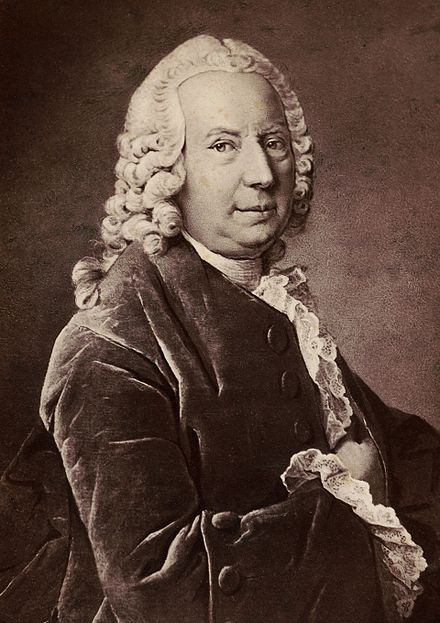
\includegraphics[width=0.8\textwidth,height=\textheight]{bernoulli.jpg}

\textbf{diminishing marginal utility} implies \textbf{risk aversion}

\end{frame}

\begin{frame}{Expected Utility Theory}
\protect\hypertarget{expected-utility-theory}{}

Humans make decisions based on \(E[U(L)]\), not \(E[L]\).

Note: \(L\) is not a variable, it is a lottery.

For example, if we define \(L\) as a lottery that pays 1 with
probability 1/2 and 10 with probability 1/2.
\(E[L] = \frac{1}{2}1 + \frac{1}{2}10 = 5.5\).

Suppose we have a log utility function. Then
\(E[U(L)] = \frac{1}{2}\ln(1) + \frac{1}{2}\ln(10) = \frac{1}{2}\ln(10) \approx 1.15\).

But \(\ln(5.5) \approx 1.7\).

So a risk averse agent prefers 5.5 with certainty to \(L\); a risk
neutral agent doesn't care.

\end{frame}

\begin{frame}{von Neumann-Morgenstern}
\protect\hypertarget{von-neumann-morgenstern}{}

Argue that expected utility = rationality. Four axioms:

\begin{enumerate}
\tightlist
\item
  Completeness: given any two things, I either prefer one or like them
  equally.
\item
  Transitivity: if I prefer A to B and B to C, I prefer A to C.
\item
  Independence of irrelevant alternatives: if I prefer A to B, I also
  prefer A+Z to B+Z (where Z is another lottery).
\item
  Continuity: there is some combination of A and B I like equally to C.
\end{enumerate}

If these hold for a person, they must be an expected utility maximizer.

\end{frame}

\begin{frame}{Arrow-Debreau Model (1954)}
\protect\hypertarget{arrow-debreau-model-1954}{}

Core way of thinking about risk:

\begin{itemize}
\tightlist
\item
  A commodity can be a thing in a certain \emph{state of the world}.
\item
  Example: today I can offer you a pupusa if it rains tomorrow. You'll
  pay a discount since rain tomorrow is unlikely.
\item
  These conditional goods are called securities.
\item
  Theoretical result: prices should exist for everything in every state
  of the world, which allows people to optimally manage risk.
\item
  Actual result: securities became very complex and buyers failed to
  understand them.
\end{itemize}

\end{frame}

\begin{frame}{Prospect Theory (1979)}
\protect\hypertarget{prospect-theory-1979}{}

Kahneman/Tversky seek to explain why real people frequently violate
expected utility theory.

Key idea: people make decisions relative to a reference point.

Rather than a concave function (risk averse everywhere), posit
risk-aversion in gains, risk-seeking in losses.

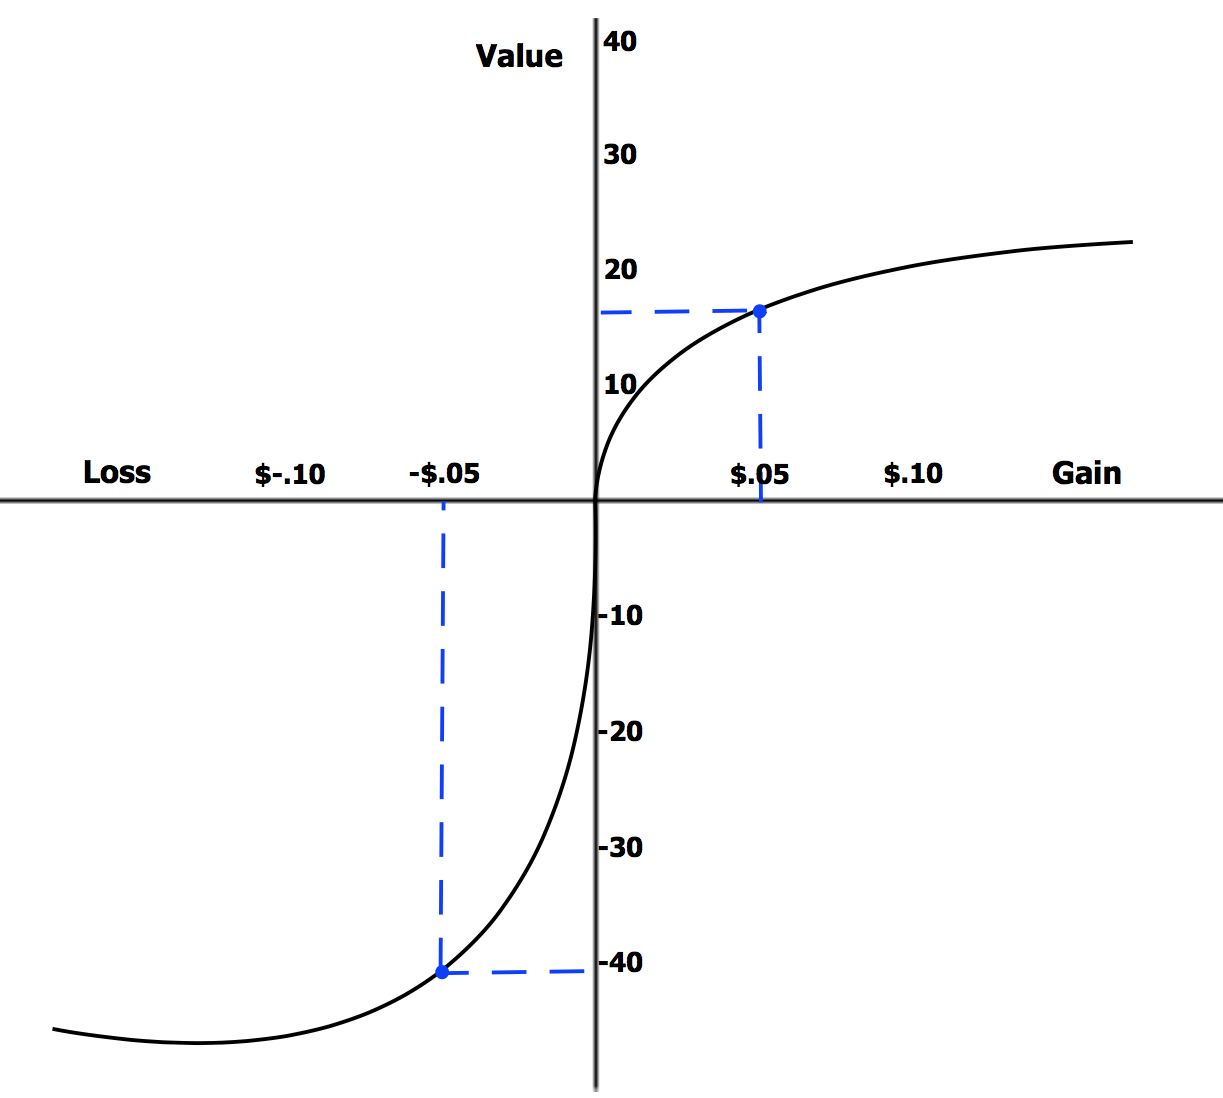
\includegraphics[width=1\textwidth,height=\textheight]{cpt.png}

\end{frame}

\begin{frame}{Prospect Theory Implications}
\protect\hypertarget{prospect-theory-implications}{}

\begin{itemize}
\tightlist
\item
  Underinvestment in insurance relative to EU (risk averse in losses).
\item
  Endowment effect
\item
  Equity premium puzzle
\end{itemize}

Problem: sometimes violates first-order stochastic dominances (predicts
choosing something that is always worse).

\end{frame}

\begin{frame}{Cumulative Prospect Theory}
\protect\hypertarget{cumulative-prospect-theory}{}

Adds probability weighting (overweighting of very likely or unlikely
events) to PT.

Idea came from Quiggin (1982). Solves first-order stochastic dominance
problem.

\end{frame}

\begin{frame}{In Summary}
\protect\hypertarget{in-summary}{}

Expected utility theory is elegant and easy to use, but people sometimes
violate it.

CPT fits some behavior better, but involves many parameters + reference
points, so it is harder to use.

\end{frame}

\hypertarget{risk-and-development}{%
\section{Risk and Development}\label{risk-and-development}}

\begin{frame}{Risk and Development}
\protect\hypertarget{risk-and-development-1}{}

Risk matters because:

\begin{itemize}
\tightlist
\item
  People in developing countries often have especially risky lives due
  to dependence on agriculture, entrepreneurship.
\item
  Macro-risks are also often greater in developing countries: currency
  risk, political risk.
\item
  Incomplete markets for credit and insurance make all of this worse.
\end{itemize}

Risk may be one of the major factors perpetuating poverty.

\end{frame}

\begin{frame}{Risk and Inequality}
\protect\hypertarget{risk-and-inequality}{}

Poor people (often) have:

\begin{itemize}
\tightlist
\item
  Less tolerance for risk
\item
  Less access to risk mitigation (credit, insurance)
\item
  Greater risk in general
\end{itemize}

This can perpetuate or exacerbate inequality (Carter + Zimmerman)

\end{frame}

\begin{frame}{Risk and Investment}
\protect\hypertarget{risk-and-investment}{}

(Uninsured) risk makes investment unappealing.

How does this connect to expected utility theory?

What different predictions might prospect theory make?

\end{frame}

\begin{frame}{How to Reduce Risk?}
\protect\hypertarget{how-to-reduce-risk}{}

\begin{itemize}
\tightlist
\item
  Social safety nets (e.g.~UBI, health insurance)
\item
  Credit
\item
  Private Insurance (but remember, moral hazard + adverse selection)
\item
  Informal Insurance
\item
  Sound macroeconomic policy + political stability
\item
  Diversified economy
\item
  Other ideas?
\end{itemize}

\end{frame}

\begin{frame}{Index Insurance}
\protect\hypertarget{index-insurance}{}

\begin{itemize}
\tightlist
\item
  Uses an index (e.g.~average regional crop yields, satellite estimates)
\item
  Pays farmers when insurance falls below threshold.
\item
  How does this affect moral hazard?
\end{itemize}

Research to date: some evidence of benefits in terms of investment +
protection, but take-up at commercially viable rates is often low.

\end{frame}

\begin{frame}{In Summary}
\protect\hypertarget{in-summary-1}{}

Risk can:

\begin{itemize}
\tightlist
\item
  Increase inequality
\item
  Increase poverty
\item
  Slow growth
\item
  Discourage investment
\end{itemize}

Reducing risk is hard, but has major benefits!

New and better ideas are needed.

\end{frame}

\end{document}
